\documentclass[12pt,english]{article}
%%% PREAMBLE

%%% Install missing packages %%%
% tinytex::parse_install("MainText.log")

% Sometimes you have to run: tinytex::install_tinytex()
% and maybe: tlmgr_update()

\usepackage{bbding} % for checkmark symbol
\usepackage{booktabs}
%\usepackage{chngcntr} % Allows table and figure counters to be reset in Appendix
\usepackage[font=small,format=hang,justification=raggedright,labelfont=up,labelsep=space,singlelinecheck=false]{caption}
\usepackage{color} % use to color text
\usepackage{enumitem}
  \setlist[enumerate]{itemsep=0mm}
\usepackage[T1]{fontenc}
\usepackage{geometry} % set margins and stuff
\usepackage{graphicx}
\usepackage{lineno}
\usepackage{longtable}
\usepackage{microtype}
\usepackage{pdflscape} % Causes pages that are in landscape format to be rotated when viewing the pdf but print as usual
\usepackage{scrextend} % Allows you to change margins for section of text
\usepackage{setspace}
\usepackage{siunitx}
\usepackage{titlesec}
\usepackage[dvipsnames]{xcolor} % use to get more colors

%\DisableLigatures{encoding = *, family = *}
\DisableLigatures[f]{encoding = *, family = *} %% <- only disables f-ligatures

\PassOptionsToPackage{hyphens}{url}\usepackage[hidelinks]{hyperref} % enables hyperlinks
\urlstyle{same} % Maintains URLs in the same font as the rest of the text

% Bibliography related
\usepackage{natbib}                            % For citations
\bibpunct{(}{)}{;}{a}{}{;}
\setlength{\bibhang}{2em}

%\addbibresource{KlibanskyFishResearch_1.5}
%\graphicspath{ {images/} }
\geometry{verbose,letterpaper,tmargin=2.54cm,bmargin=2.54cm,lmargin=2.54cm,rmargin=2.54cm}
%\linenumbers

\captionsetup{figurename=Fig.}

% Define heading formatting
\titleformat{\section}
   {\small\mdseries\scshape}{\thesection}{1em}{}

\titleformat{\subsection}
   {\small\mdseries\itshape}{\thesubsection}{1em}{}

\titleformat{\subsubsection}
   {\small\mdseries}{\thesubsubsection}{1em}{}

%%% Main document
% BEGIN DOCUMENT
\usepackage{Sweave}
\begin{document}
\Sconcordance{concordance:MainText.tex:MainText.Rnw:%
1 56 1 1 0 2 1 1 9 1 11 1 5 1 14 273 1}









% Top matter
\title{Evaluating procedures for updating catch advice between stock assessments of reef fishes with management strategy evaluation}
\author{Nikolai Klibansky,  Shannon Calay, Rob Cheshire,\\
Cassidy Peterson, Kyle Shertzer, Erik Williams, and Matt Vincent\\\\
Southeast Fisheries Science Center, \\
National Marine Fisheries Service, NOAA,\\
101 Pivers Island Road, Beaufort, North Carolina, 28516, USA}
\maketitle

\begin{abstract}
We conducted a management strategy evaluation (MSE) to investigate how management procedures that adjust catch advice between stock assessments performed compared with existing management procedures. We built operating models (OM) for four reef fish species from the US Southeast Atlantic, based on recent stock assessments including Black Sea Bass, Red Porgy, Snowy Grouper, and Vermilion Snapper. These OM contained parameters and data specific to each stock, associated fisheries, and the sampling programs that monitor them. The analysis assumed efficient implementation of management, such that observed catch was equal to total allowable catch (TAC). Our analysis focused on a base scenario intended to most closely characterize the reality of each stock. We also developed multiple alternative scenarios to investigate the sensitivity of the analysis to deviations from the base configuration. A set of management procedures (MP) was applied independently in closed loop simulation for each species and scenario, with many replicate runs. The MP varied in terms of how often stock assessments were conducted (every 1, 5, or 10 years), and how catch advice (i.e. TAC) was adjusted between stock assessments. Between assessments, TACs were either fixed, adjusted based on projections, or adjusted based on a reference index of abundance. Results varied among species and scenarios, but generally showed that healthy stock and fishery status ($\mathrm{SSB>SSB_{MSY}}$ and $F<F_{\mathrm{MSY}}$) and comparable levels of total catch could be maintained with stock assessments conducted every 1, 5 or 10 years, whether TACs were fixed, projected, or adjusted based on indices of abundance. But these management procedures vary in terms of average annual variability in yield (AAVY) which was highest when TACs were adjusted based on indices of abundance and lowest when TACs were fixed between assessments.

\end{abstract}

\begin{flushleft}
\begin{spacing}{1.9}
\setlength{\parindent}{1cm} % Indent paragraphs after the first one

\section*{Introduction}

\subsection*{Motivation}
Stock assessments are highly resource intensive processes. Recent NMFS guidance has prioritized increasing assessment throughput and reducing assessment frequency where appropriate for managed species (\citealt{ICES2012}; \citealt{Methot2015}; \citealt{LynchEtAl2018}). Reduced stock assessment frequency would free up assessment scientists to conduct research to advance fisheries management and prioritize unassessed stocks.

One such mechanism of allowing reduced stock assessment frequency while still providing continuous adaptive management is through the use of interim assessment approaches \citep[e.g., ][]{HuynhEtAl2020}. Interim assessment approaches use an indicator of stock abundance (e.g., index of abundance) to adjust total allowable catch (TAC) between full stock assessments. Interim assessments would still require updated data and analytical input from assessment scientists, but the computational load and time commitment would be substantially diminished. Interim assessments have been found to be conceptually sound (Huynh et al. 2020), and here we seek to identify whether these methods are suitable for stocks in the South Atlantic.

\subsection*{MSE Background}
The current stock assessment paradigm and the interim assessment approach are each examples of a management procedure. A management procedure, or management strategy, is a formal rule that defines how fisheries are managed and includes (1) a clearly defined data-generating protocol, (2) an estimating model that describes the current state or condition of the stock (e.g., stock assessment), (3) a predefined catch (harvest) control rule that describes how catch advice should be adjusted given the state of the stock, and (4) an implementation rule which describes how the catch advice will be applied (\citealt{SainsburyEtAl2000}; \citealt{Punt2010}). Management procedures are designed to be adaptive to changes in stock biomass or trajectory (e.g., as estimated biomass declines, allowable catch declines; \citealt{Edwards2016}). Consider how the current assessment paradigm can be presented within the management procedure framework, for example, as it includes: (1) a data-collection enterprise to collect abundance, biological, and catch information from the stock; (2) the stock assessment, or estimating, model which uses scientifically collected data to provide an estimate of stock status and biological reference points, (3) catch control rule, which varies with each FMC, but examples include the $P*$ approach \citep{ShertzerEtAl2008} or the 40-10 rule \citep{PFMC2020}, and (4) the implementation of the catch control rule-defined management action, often in the form of TACs.

Because in situ scientific testing of alternate management procedures is logistically unfeasible in practice, we test management procedures using management strategy evaluation (\citealt{ButterworthPunt1999}; \citealt{DeOliveiraEtAl2008}). MSE is a framework for testing candidate management procedures across a range of uncertainties using closed-loop simulation (Fig. \ref{fig:diagram}; \citealt{Holland2010}; \citealt{PuntEtAl2016}).

Management procedure performance is measured based on pre-specified performance metrics, which are designed to reflect the management objectives of the system. Typically management objectives include increasing total allowable catch and reducing risk to the resource. When management objectives are not already defined, as in a Fishery Management Plan, stakeholder involvement is often necessary to clarify the goals of the fishery. Understandably, not all performance metrics can be simultaneously maximized (e.g., increasing TAC increases risk to the resource). MSE therefore serves to lay bare the societal trade offs associated with fisheries management \citep{Punt2017}.

An operating model is created that represents the 'true' system dynamics, and the full management procedure is applied to the stock(s) of interest simulated in the operating model. However, there are many assumptions that must be made when generating a simulation of a stock and fishery. To ensure that none of these assumptions or decision-points impact the results, particularly those that are most uncertain, multiple operating models can be generated representing different scenarios (\citealt{ButterworthPunt1999}; \citealt{DeOliveiraEtAl2008}; \citealt{PuntEtAl2016}). For example, if natural mortality is uncertain, multiple scenarios can be built with different realistic assumptions of natural mortality (high, medium, and low).

We then measure the effects of the management procedure on the 'true' populations simulated by the operating models. If the management procedure cannot perform well across all operating models (e.g., natural mortality scenarios), then it likely is not a good candidate for implementation, because we are unlikely to know the real natural mortality rate in practice. The presence of multiple operating models serves as a test of the management procedure against many possible realities, ensuring that the chosen management procedure is robust to the uncertainties that we have in the system (\citealt{ButterworthPunt1999}; \citealt{RademeyerEtAl2007}; \citealt{PuntEtAl2016}). These uncertainties can extend to future projections, accordingly monitoring how management procedures would perform in the face of nonstationarity.

\subsection*{Interim assessment approach}
	While setting interim-period catches based on assessment model forecasts can yield improved performance over fixed catches, \citet{HuynhEtAl2020} noted that forecasts are made under assumptions of future stock dynamics and are not responding to true observed changes in stock size. The interim approach is a modification of an empirical, indicator-based management procedure, in which catch advice is adjusted based on an indicator of stock abundance (e.g., index of abundance; \cite{GeromontButterworth2015}; \cite{CarruthersEtAl2016}). Within the interim approach, TACs set by the stock assessment model are adjusted in interim years based on the behavior of the stock indicator. Unlike traditional stock assessment-based TACs, interim assessment TAC adjustments may be implemented immediately with no time-lag \citep{HuynhEtAl2020}.

\citet{HuynhEtAl2020} used MSE to test the interim assessment approach across 3 species of differing life histories (short-, moderate-, long-lived), each with 6 unique operating model scenarios (Base, Hyperstable, Hyperdeplete, Depleted, Lightly fished, Episodic M), using the openMSE software suite [openMSE, \cite{openMSE}; DLMtool, \cite{DLMtool}; MSEtool, \cite{MSEtool}; SAMtool, \cite{SAMtool}]. Authors found that the use of an interim assessment approach markedly improved management performance over using a fixed TAC between assessments and more closely approximated the management performance of using assessment projections to specify interim period catches. Furthermore, management resulting from the interim assessment approach was not adversely impacted by increased interim period length and hyperstable/deplete scenarios in which the assumption that the relative abundance index is proportional to stock biomass is violated. Ultimately, the interim approach reduced the need for frequent stock assessments, potentially freeing up resources to focus on other stocks or research questions.

\subsection*{Study Objectives}
In this study, we sought to replicate the \citet{HuynhEtAl2020} approach by applying it specifically to South Atlantic fishes based on information from the most recent stock assessments. Representative species analyzed include Black Sea Bass, Red Porgy, Vermillion Snapper, and Snowy Grouper. We used species-specific biological parameters and were able to more accurately describe the data-generating, fishery, and stock assessment dynamics for these species within the openMSE framework, including delays in data collection and management implementation \citep{ShertzerPrager2007} and specification of different selectivity functions for catch and abundance indices. Simulations were further specified with empirically estimated levels of observation and process uncertainty. The purpose of this study was to explore whether interim assessment approaches would be suitable for South Atlantic fishes.

\section*{Materials and Methods}

\subsection*{Operating models}
We used the most recent stock assessments from US Southeast US Atlantic for Red Porgy \citep{SEDAR60}, Black Sea Bass \citep{SEDAR56}, Vermilion Snapper \citep{SEDAR55}, and Snowy Grouper \citep{SEDAR36Update}. Elements of the stock assessments are stored as data sets in the R package \texttt{bamExtras} (\url{https://github.com/nikolaifish/bamExtras}). Management strategy evaluation was conducted with the R package \texttt{openMSE} \citep{openMSE}, which includes three sub-packages \texttt{DLMtool}, \texttt{MSEtool}, and \texttt{SAMtool} (\citealt{DLMtool}; \citealt{MSEtool}; \citealt{SAMtool}). This package uses a set of data objects with very specific list-like structures (S4; \url{http://adv-r.had.co.nz/S4.html}), such as operating model objects (\texttt{OM}). Such objects are made up of a set of named 'slots', which contain specific types of information with particular dimensions, to characterize main components of an MSE. Input and output from the Beaufort Assessment Model (BAM) is configured as a list which has a specific structure, and is stored in an \texttt{rdat} file. The most recent \texttt{rdat} files are also stored in \texttt{bamExtras} as objects (e.g. \texttt{rdat\_BlackSeaBass}). In order to the transfer information from BAM \texttt{rdat} objects to \texttt{openMSE} objects, we wrote a set of functions and constructed a new R package, \texttt{bamMSE} (\url{https://github.com/nikolaifish/bamMSE}).

Operating models in \texttt{openMSE} (\texttt{OM} class S4 objects) are constructed of four sub-objects: \texttt{Stock}, \texttt{Fleet}, \texttt{Obs}, and \texttt{Imp} class objects. Values stored in \texttt{Stock} objects describe a fish stock, \texttt{Fleet} objects characterize a fishing fleet that fishes that stock, \texttt{Obs} objects contain parameters describing how the simulated stock and fleet are observed (e.g. bias and error of catch or relative abundance data), and the \texttt{Imp} objects allow the user to set how well managers adhere to management recommendations (i.e. implementation error). A fifth \texttt{openMSE} object class \texttt{Data}, is used to store various types of data, including data sets typically used in fitting stock assessment models (e.g. indices of abundance, catch, and age-composition time series). Functions in \texttt{bamMSE} convert \texttt{rdat} objects to \texttt{Stock}, \texttt{Fleet}, \texttt{Obs}, and \texttt{Data} objects (\texttt{rdat2Stock}, \texttt{rdat2Fleet}, \texttt{rdat2Obs}, and \texttt{rdat2Data}).

We used the function \texttt{MSEtool::Assess2OM} to convert BAM results to \texttt{OM} objects, with the help of a wrapper function \texttt{bamAssess2OM} (not yet added to \texttt{bamMSE}). While the values of the steepness parameter $h$, and unfished recruitment ($R_{0}$) for the Beverton-Holt stock-recruit relationship are directly passed from BAM to \texttt{Assess2OM}, most other inputs had to be modified from BAM. Since \texttt{openMSE} requires the first age in age-structured populations to be age-0 and most BAM assessments start with age-1, age-based data from BAM was linearly extrapolated from age-1 to age-0 before being passed to \texttt{Assess2OM}. Such data include several three dimensional numeric arrays with dimensions simulation, age, and year (within recent assessment period): fish weight, fish length, proportion mature, numbers of fish, total fishing mortality rate ($F$; including dead discards) , and natural mortality rate ($M$).

Maturity-at-age is used to compute spawner biomass using methods followed in BAM assessments. For gonochoristic species (separate male and female sexes; Vermilion Snapper) maturity-at-age was based on females. For protogynous hermaphrodite species (females transition to male as they age; Black Sea Bass, Red Porgy, and Snowy Grouper) maturity-at-age was based on the proportion of fish of either sex mature-at-age.

We ran  \texttt{rdat2Data} on the \texttt{rdat} objects, and passed indices of abundance, their associated CVs, and selectivity-at-age to an \texttt{openMSE} \texttt{cpars} list object. In \texttt{openMSE} a \texttt{cpars} list object is used to pass custom parameters, typically time-varying, to an operating model. The \texttt{rdat2Data} function assumes that indices based on surveys or recreational fisheries are in numbers and indices based on commercial fisheries are in pounds. Only indices available in the terminal year of the assessments were passed to \texttt{cpars} and the \texttt{OM} objects (Fig. \ref{fig:AddInd}). Estimates of growth parameters ($K$, $L_{\infty}$, and $t_{0}$) from BAM were also passed to the \texttt{OM} objects. Selectivity-at-age of removals is estimated annually during the empirical assessment period by \texttt{Assess2OM}, and the average of the last three years of the assessment period was passed to \texttt{cpars} and the \texttt{OM} objects to be used in the projection years.

In most cases, empirical values provided to the \texttt{OM} objects are used to determine distributions of parameters, data, or residuals. These distributions are then used by \texttt{openMSE} when simulating values in the projection years. For example, the number of age samples (numbers of otoliths) available to management procedures during the projection period are determined by drawing from a distribution based on how many age samples were actually available in the most recent SEDAR assessment of that species. However, the time series of residuals for indices of abundance, were generated ahead of time and added to the \texttt{OM} objects. Residuals were sampled from a lognormal distribution based on index CVs from the most recent SEDAR assessment. In the base and most other scenarios, life history parameters were constant over time in the simulated populations. Maximum $F$ was limited in the simulations by rounding the maximum observed $F$ up to the next integer value. This limit prevents catch limits from being set unreasonably high.

\subsection*{Management procedures}

The entire MSE was run repeatedly and independently, applying one of nine different management procedures (MP). In all of these MP, age-structured stock assessments were conducted at a frequency of every 1, 5, or 10 yr. For all MPs, in an assessment year, reference points were estimated (e.g. $\mathrm{MSY}$, $F_{\mathrm{MSY}}$), and a simple harvest control rule was applied to determine the TAC for the following year. The TACs were computed from the assessment output using the \texttt{SAMtool::HCR\_MSY} function which projects abundance one year beyond the terminal year of the assessment, and applies the catch equation used in the assessment and the target level of fishing mortality ($F_{\mathrm{target}}$). In the base scenario, $F_{\mathrm{target}}$ was set equal to $F_{\mathrm{MSY}}$ from the simulated assessment. We also limited the maximum $F$ to $F_{\mathrm{max}}=3$ to avoid simulating unreasonably high catch levels. Between assessments, catch was set in different ways.

In the fixed TAC MPs [SCA (1), SCA (5), and SCA (10)] stock assessments were conducted every 1, 5, or 10 yr respectively, and the harvest control rule was applied to determine the TAC. Between assessments, the TAC was fixed.

In the projection MPs, [Projection (5) and Projection (10)], stock assessments were conducted every 5 or 10 yr, respectively. In these MPs a projection analysis is simulated in order to set the TACs for the interval between assessments. The population is projected forward for the interval between assessments $F_{\mathrm{target}}$ is applied to compute catch. These catches are then used as TACs in the simulated management during the interval. These TACs will tend to exhibit a temporal trend since projected abundance is not usually constant.

In the average index interim MPs [Average Index (5) and Average Index (10)] stock assessments were conducted every 5, or 10 yr respectively. In an assessment year, the TAC is computed as in other MPs, and is treated as a reference catch ($C_{\mathrm{ref}}$) in the interim procedure. The value of a selected index of abundance is also recorded and treated as a reference value ($I_{\mathrm{ref}}$). Between assessments, a TAC in year $y+1$ is set by  according to Eq. \ref{eq:iMPavg}:

\begin{equation}
\mathrm{TAC}_{y+1} = C_{\mathrm{ref}}\frac{\tilde{I}_{\mathrm{recent}}}{I_{\mathrm{ref}}}
\label{eq:iMPavg}
\end{equation}

This calculation scales $C_{\mathrm{ref}}$ by the ratio of an average of the three most recent years of the abundance index ($\tilde{I}_{\mathrm{recent}}$) and the reference year ($I_{\mathrm{ref}}$). Using the average of recent years of the index instead of a single recent value effectively smooths the index. This serves to avoid a noisy index leading to highly varying TACs.

In the buffered index interim MPs, Buffered Index (5) and Buffered Index (10), stock assessments were conducted every 5, or 10 yr respectively. Between assessments, a TAC in year $y+1$ is set by  according to Eq. \ref{eq:iMPbfr}:

\begin{equation}
\mathrm{TAC}_{y+1} = C_{\mathrm{ref}} \frac{I_{y} + \hat{\sigma}}{I_{\mathrm{ref}} + \hat{\sigma}}
\label{eq:iMPbfr}
\end{equation}

where $I_{y}$ is the value of the index in the most recent year and $\hat{\sigma}$ is the standard deviation of the index. Including $\hat{\sigma}$ in this calculation assures that the noisier the index, the smaller the adjustment to the TAC, limiting variation in TACs.


% \begin{enumerate}
% \setstretch{1}
% \item Average catch (AvC): Average catch over all years
% \item Recent catch (CC1): Average catch over the last 5 years
% \item Depletion corrected average catch (DCAC):
% \item Depletion based stock reduction analysis (DBSRA):
% \item Surplus production model (SPMSY):
% \item Statistical catch-at-age model
% \begin{enumerate}
% \item 1-year interval (SCA (1))
% \item 5-year interval with fixed TAC between years (SCA (5))
% \item 10-year interval with fixed TAC between years (SCA (10))
% \item 5-year interval with projected TAC between years (Projection (5))
% \item 10-year interval with projected TAC between years (Projection (10))
% \item 5-year interval with TAC adjusted based on averaged recent index between years  (Average Index (5))
% \item 10-year interval with TAC adjusted based on averaged recent index between years  (Average Index (10))
% \item 5-year interval with TAC adjusted based on buffered averaged recent index between years  (Buffered Index (5))
% \item 10-year interval with TAC adjusted based on buffered averaged recent index between years  (Buffered Index (10))
% \end{enumerate}
% \end{enumerate}
% \setstretch{2}

\subsubsection*{Statistical catch-at-age model configuration}

Management procedures that ran statistical catch-at-age models utilized the \texttt{SAMtool::SCA} function. The model run in this function was configured as similar to BAM as the function would allow. The configuration was specific to each species' operating model where applicable.
% Data structure

The range of ages modeled in the assessments is from age-0 to the maximum age modeled in the BAM assessment for each species. Life history is age-structured such that, length, weight, maturity, and natural mortality vary with age. Years of data included in the time series span from the earliest historical year to two years prior to the current year (i.e. assessment year).  Management changes go into effect the year following the assessment. Effectively, the last two years of available data are excluded from the stock assessment, to simulate a typical data lag observed in SEDAR assessments. For interim procedures, we assumed that management would be put in place the next year, and therefore did not impose any additional data lag. Applying data lags is not a standard option in \texttt{openMSE} so the lag option was written into wrapper functions for \texttt{SAMtool} functions \texttt{SCA}, \texttt{make\_MP}, \texttt{make\_interim\_MP}, and \texttt{make\_projection\_MP}, for this project.

The \texttt{SCA} models included one combined set of removals (landings and discards). Although most of the empirical BAM assessments include multiple fleets of removals with landings and discards separate, this is not an option when using \texttt{runMSE}\footnote{The flexibility to add multiple landings fleets has recently been added to \texttt{openMSE} using the \texttt{multiMSE} function, but would require a nontrivial amount of coding to incorporate into the current analysis.}. The model also fits to one or more indices of abundance, depending on the species, and one set of simulated catch-at-age data corresponding to the landings.


% Selectivity
Selectivity-at-age associated with removals was estimated within \texttt{SCA} with a logistic selectivity function. Selectivity of the indices was provided to \texttt{SCA} as fixed information.

The \texttt{SCA} model used a Beverton-Holt stock-recruit function, the Baranov catch equation, and a multinomial distribution for fitting catch-at-age information. Several parameters are fixed by default in \texttt{SCA} including Beverton-Holt steepness, equilibrium $F$, CV associated with catch, and the standard deviation of recruitment residuals (i.e. "rec sigma"). Recruitment deviations were estimated for one generation prior to the first year that age-composition data were available. Toward the end of each assessment, recruitment deviations were not estimated for several years and recruitment was predicted from the mean value of the stock-recruit relationship. The number of years for which recruitment deviations were not estimated was based on an option within the \texttt{SCA} function (\texttt{late\_dev="comp50"}) which specifies it as the: ``number of ages (smaller than the mode) for which the catch-at-age matrix has less than half the abundance than that at the mode'' (\texttt{SAMtool::SCA} help file).

\subsection*{Scenarios}

The configuration of the MSE described above was considered the base scenario. Various modifications to the configuration were made to create other scenarios described below. Many other scenarios were explored but did not change the conclusions of our analysis, so they are not included in the current report.

\begin{enumerate}
\setstretch{1}
\item Index high CV (ucvhi): Uncertainty (coefficient of variation; CV) in primary index of abundance of abundance is twice the CV of the base scenario
\item Index low CV (ucvlo): Uncertainty (CV) in primary index of abundance of abundance is half the CV of the base scenario
\item Index is biased (ubias): Primary index of abundance increasingly underestimates population size (i.e. decreasing catchability)
\item High TAC (tachi): TAC = 1.25MSY ($F_{\mathrm{target}} = 1.25F_{\mathrm{MSY}}$ in harvest control rule)
\item Low TAC (taclo): TAC = 0.75MSY ($F_{\mathrm{target}} = 0.75F_{\mathrm{MSY}}$ in harvest control rule)

% \item Base (base): Most likely scenario, described above
% \item Depleted (dep): Depletion of the stock is high (i.e. smaller stock size) at the beginning of the projection period
% \item Lightly fished (lf): Depletion of the stock is low (i.e. larger stock size) at the beginning of the
% \item Regime change (rc): Recruitment deviations decline over the projection period, then remain low
% \item Minimal error (minerr): Minimal (but not zero) error in all stochastic elements of the \texttt{OM}
% \item Minimal rec. dev. (minrecdev): Recruitment deviations set to low value
% \item Non-stationary recruitment (recns)
% \item Vulnerability time invariant (vtiv): Selectivity associated with catch (i.e. vulnerability) does not vary annually during the historic period.
%
% \item No empirical indices (noempind): No empirical indices, CVs, or index selectivities are included in the \texttt{OM}
% \item Catch CV 0.05 (catcvlo): CV of catch is set to 0.05 when fitting to catch in stock assessments.
% \item No data lag (nolag): Catch advice (i.e. TAC) from stock assessments is implemented the year after the terminal year of the assessment
% \item Perfect observation (perfobs): Minimal observation error and very high sample sizes in data sets
%
% \item Set life history (lhset): $M$ and $h$ are set to the same fixed values for all species ($M$ = 0.2, $h$ = 0.84)
% \item Set $M$ (Mset): $M$ is set to the same fixed value for all species ($M$ = 0.2)
% \item Set $h$ (steepset): $h$ is set to the same fixed value for all species ($h$ = 0.84)
% \item Age-varying $M$ (agevarM): $M$ varies with age
% \item Episodic $M$ (epiM): $M$ is constant in most years but is occasionally much higher

% \item Hyper-deplete: Primary index of abundance is hyper-deplete
% \item Hyper-stable: Primary index of abundance is hyper-stable
% \item Vulnerability dome-shaped (vdome): Selectivity associated with catch (i.e. vulnerability) is estimated with a dome-shaped function in stock assessments

\end{enumerate}
\setstretch{2}


For each management procedure, we ran the replicate simulations 250 times for the base scenario and 50 times for each alternative scenario. In preliminary analysis of the base scenario, we found that results were approximately the same with 50 runs as 250 runs, although output plots were smoother when more runs were completed. However, output objects from 250 are rather large (200-400 Mb) and become cumbersome to work with.

\subsection*{Evaluating performance}
To evaluate the relative performance of the MPs, we consider a set of reference points and performance metrics. We computed total catch, relative catch ($C/\mathrm{MSY}$), stock status ($\mathrm{SSB/SSB_{MSY}}$), fishery status ($F/F_{\mathrm{MSY}}$), and the average annual variability in yield (AAVY). The AAVY is the absoluted relative difference in catch between two consecutive years, calculated as in Eq. \ref{eq:AAVY}:
\begin{equation}
\mathrm{AAVY} = \frac{\sum_{y=1}^{Y}\sqrt{(\frac{C_{y}-C_{y+1}}{C_{y+1}})^{2}}}{Y}
\label{eq:AAVY}
\end{equation}
where $C_{y}$ and $C_{y+1}$ are catches in years $y$ and $y+1$, and $Y$ is the total number of years in the projection period.

We also computed several performance metrics, focusing on long term values, measured during the last 10 years of the projection period. These included average long term yield, the probability [$\mathrm{P()}$] of healthy stock status $\mathrm{P(SSB>SSB_{MSY})}$, the probability of not overfishing $\mathrm{P}(F<F_{\mathrm{MSY}})$, and the probability of stable yield $\mathrm{P(AAVY<20\%)}$.

\section*{Results}

\subsection*{Base scenario}

% Boxplots
Response variables for the base scenario varied among time periods over the projection years for all metrics. Stock status ($\mathrm{SSB/SSB_{MSY}}$) increased over time among all nine SCA-based MPs for all four species, but was similar between MPs during the same time interval (Fig. \ref{fig:boxplotSBSBMSY1}). Fishery status ($F/F_{\mathrm{MSY}}$) was somewhat more  variable within and between MPs, but still largely consistent among SCA-based MPs, for all species (Fig. \ref{fig:boxplotFFMSY1}). Total catch was also similar among SCA-based MPs for all species, for similar time periods (Fig. \ref{fig:boxplotCatchTotal1}). It was relatively less consistent for Black Sea Bass, but variability in total catch within MPs was also more variable for that stock. Average annual variability in yield (AAVY) showed more substantial variation among MPs (Fig. \ref{fig:boxplotAAVY1}). For Vermilion Snapper and Snowy Grouper, the fixed TAC and projection MPs showed substantially lower AAVY than the interim MPs. Red Porgy showed a similar pattern, although AAVY for the Average Index (5) and Average Index (10) was relatively lower. For Black Sea Bass, there was relatively little difference in AAVY among MPs compared to the other species.

% Time series plots
Time series of relative catch (catch/MSY), averaged across simulation runs, are generally most stable when assessments are run annually, and show the largest interannual variations when projection MPs are used (Figs. \ref{fig:tsCatchMSY1} and \ref{fig:tsCatchMSY1B}). For the projection MPs, the difference in catch between consecutive years is actually modest for most years, but tends to be very large between a stock assessment year and the next year, leading to periodic spikes. For Black Sea Bass, the fixed TAC MP was often well above or below the other MPs with a 10 yr assessment interval, but catches were otherwise very steady because TACs were fixed during the intervals. The index-based approaches tended to produce similar catches which were more consistent than the projection and fixed TAC MPs. Relative catches were all more similar to the annual assessment MP when the assessment interval was 5 yrs. Patterns in $F/F_{\mathrm{MSY}}$ time series reflected dynamics similar to the catch. However the fluctuations in the projection MP were less pronounced (Figs. \ref{fig:tsFFmsy1} and \ref{fig:tsFFmsy1B}) and tended to be lower than other MPs, representing a more conservative strategy. Despite differences in catch and relative $F$ among MPs, trends in $\mathrm{SSB/SSB_{MSY}}$ were similar among all MPs for Red Porgy and Snowy Grouper. For Vermilion Snapper only the projection MP deviated from the others, with $\mathrm{SSB/SSB_{MSY}}$ tending to be slightly higher (Figs. \ref{fig:tsSSBSSBmsy1} and \ref{fig:tsSSBSSBmsy1B}). Trends in $\mathrm{SSB/SSB_{MSY}}$ for Black Sea Bass varied among MPs with a 10 yr assessment interval, with the Fixed TAC MP showing the widest fluctuations. But with a 5 year assessment interval, $\mathrm{SSB/SSB_{MSY}}$ trends were fairly similar among MPs for all species including Black Sea Bass.

% Trade off plots
Trade off plots display bivariate relationship between two performance metrics for multiple management procedures, to identify differences between MPs in performance-metric space. We considered several important trade offs to look for differences in performance among MPs, plotting mean values across simulation runs, for each MP. In particular we looked at trade offs between yield (catch), variability in yield, or fishery status, versus stock status. We limited data used to produce these plots to the final 10 years of the projection, to look at long term values.

Trade off plots of probability that AAVY < 20\% versus the probability that $\mathrm{SSB>SSB_{MSY}}$ (Fig. \ref{fig:trAAVYP1001}), the probability that $F<F_{\mathrm{MSY}}$ (Fig. \ref{fig:trAAVYPNOF1}), and mean relative long term yield (Fig. \ref{fig:trAAVYYldLT1}), show little differentiation among MPs along the vertical axis. The MPs mostly differ in the probability of that AAVY < 20\%. As suggested in other plots, SCA (5), and SCA (10) produce more consistent yields, which is indicated in trade off plots as having higher probabilities that AAVY < 20\%. Performance of other MPs in terms of probability of AAVY < 20\% varied by species. Trade off plots of mean relative long term yield versus the probability that $\mathrm{SSB>SSB_{MSY}}$ (Fig. \ref{fig:trP100YldLT1}) and probability that $F<F_{\mathrm{MSY}}$ versus probability that $\mathrm{SSB>SSB_{MSY}}$ (Fig. \ref{fig:trPNOFP1001}) do not indicate any consistent differentiation among MPs.

% Phase plots
We also produced phase plots of $F/F_{\mathrm{MSY}}$ versus $\mathrm{SSB/SSB_{MSY}}$ (Fig. \ref{fig:phasePlot1}) including median values among all simulation runs, as well as points for each run. Again we limited data to the final 10 years of the projection periods. Phase plots also do not indicate any consistent differentiation among MPs. However the projection MP resulted in slightly higher stock status for Vermilion Snapper and Red Porgy and the fixed TAC MP resulted in slightly higher $F$-status in Black Sea Bass.

\subsection*{Alternative scenarios}
Although results for alternative scenarios differed from the base in various ways, the overall results are the same (Figs. \ref{fig:boxplotSBSBMSY2}-\ref{fig:phasePlot2}). Management procedures perform similarly except for variation in variability of catch. One exception to this generality is for Red Porgy in the scenario where the harvest control rule set the TAC to $1.25\times\mathrm{MSY}$. Under this scenario, the Red Porgy could not recover from its already depleted state and only the annual assessment MP was able to keep the stock from going completely crashing in more than 50\% of simulation runs (Fig. \ref{fig:phasePlot2}).

\section*{Discussion}

Overall, our analysis suggested that all of the management procedures we considered resulted in similar trends in $\mathrm{SSB/SSB_{MSY}}$ for a given stock and scenario. With a 10 yr assessment interval the Black Sea Bass stock, showed the most variability among MPs, and only the annual assessment MP produced stable $\mathrm{SSB/SSB_{MSY}}$ until late in the projection period; but with 5 yr assessment intervals, all MPs produced similar results. In this stock the projection MP tended to be a bit conservative, resulting in fairly high $\mathrm{SSB/SSB_{MSY}}$, but even this MP could be tuned by applying a more aggressive harvest control rule if that was desired.

Even this variation in $\mathrm{SSB/SSB_{MSY}}$, evident in the central tendency of the time series, is less apparent when comparing distributions in boxplots by time period. This is generally true for $F/F_{\mathrm{MSY}}$ as well. Distributions of total catch are also similar among MPs, comparing the same time periods.

The performance metric that really separates the MPs is variability in yield. The simplest, fixed TAC, MPs correspond to the lowest variability in yield, followed by the projection MPs which set TACs that change between assessments but follow a simple trajectory. For the index-based approaches, TACs vary in more complex ways between assessments based on changes in abundance, leading to greater variability in catch.

An ideal interim management procedure would allow for stock assessments to be conducted less frequently while still achieving management goals. While we found index-based interim MPs performed somewhat better than fixed TAC MPs when comparing time series of $\mathrm{SSB/SSB_{MSY}}$ at the assessment frequency, there is no clear improvement when comparing interim procedures conducted with an assessment frequency of 10 yrs and fixed TAC MPs with a assessment frequency of 5 yrs.

It may be possible to improve upon the index-based MPs, although we did not investigate this. In particular, the computation used to adjust the TACs can be easily modified to decrease variation in TACs and presumably catch. But it's likely that this modification would trade off with the ability of the MP to maintain desirable stock status. Such an MP might be expected to occupy a location in performance space intermediate between the current index-based MPs and the fixed TAC MPs.

In order for a new MP to be favored over and existing one, it would likely need to exhibit a more favorable ratio of performance to effort. We have focused on assessing performance, but can make some basic conjectures about effort that might be useful to guiding decisions about whether or not interim procedures are favorable. If we assign 1 unit of scientific effort to conducting a stock assessment (including analysis and process; e.g. SEDAR), then conducting one assessment every 5 years would be 0.2 units per year (upy) and every 10 years would be 0.1 upy. If an index-based TAC adjustment were to be applied every year, it would be completed nine times in 10 years. Therefore the relative effort of completing such an analysis was equal to 0.1/9 upy, it would take just as much effort as doing one additional assessment, and therefore the effort would be equivalent to doing assessments every 5 years. It is likely that the analytical effort of updating an index of abundance and applying the adjustment procedure is substantially less than the effort that goes into an entire assessment, and presumably the assessment process would be simpler. But it seems less clear that the effort would be less than $\frac{1}{9}^{\mathrm{th}}$ as much.

In addition, we should consider the management effort required to review and adjust catch advice, similarly assigning 1 unit of management effort per assessment and 0.2 upy when conducting assessments every 5 years. But in this case, the management effort required to review and adjust catch advice based on an updated index is probably similar to the management effort of a full assessment. Therefore the management effort of applying an index-based MP with an assessment interval of 10 years would be about 1 upy, or about $5\times$ the management effort of applying a fixed TAC or projection MP with an assessment interval of 5 years.

This consideration of effort is clearly hypothetical, but attempts to outline some of the costs that an index-based MP might have to overcome to be preferred over the status quo approach. In the present analysis we found limited improvement of the index-based MPs over status quo approaches in terms of maintaining healthy stocks, and poorer performance in terms of more variable catches. So if the net performance of the index-based MPs could even be considered similar to the status quo, the actual effort associated with conducting and implementing an index-based MP will have to be very low for the approach to be preferred.



% Potential discussion materials from Quang's paper:
% Areas of future interim MP research:
% - Can tune interim MP to meet specific performance objectives
% - Future case-studies can evaluate how interim MPs perform if survey and fishery vulnerability are substantially different
% - Changes in environmental conditions may require revision of reference points
% - Model misspecification
% - Further evaluation of the interim MPs will need to account for the time lags in the management system.


% Which factors seem to account for the most variation in results in general?
% \begin{itemize}
% \item Above all, results differ between operating models (i.e. species)
% \item Scenario is the next most important factor, particularly depletion scenarios and regime change
% \end{itemize}

\section*{Acknowledgements}
We extend special thanks to Quang Huynh for answering many questions about the \texttt{openMSE} software and writing new features and functions into the software in response to our inquiries. Thanks also to Adrian Hordyk and Tom Carruthers at Blue Matter for additional help with \texttt{openMSE}. Thank you to Kate Siegfried and Lew Coggins for thoughtful suggestions. Thanks to the Fischmeister 5000 uber computer for running computations day and night, without complaint.

\end{spacing}
\end{flushleft}

% \printbibliography
%%% LITERATURE CITED %%%
%\printbibliography
\clearpage
\section*{Literature Cited}
\renewcommand{\refname}{}
\bibliographystyle{ecosphere} % Modified from ecology.bst
\vspace{-1cm}

\bibliography{KlibanskyFishResearch_1.5}


%% TABLES
% \newpage
% \section*{Tables}

%\input{../Results/biodivByArea.tex}
%\clearpage


%% FIGURES %%
\newpage
\section*{Figures}

% Indices
\begin{figure}[!ht]
\begin{center}
\includegraphics[width=6in,height=5.25in]{../Figs/MSEDiagram.png}
\end{center}
\begin{flushleft}
\caption{Diagram of the MSE process. The operating model is the simulated "true" dynamics of the system; the observation, or data-generating, model simulates the process of scientific data collection from the stock and fishery; the estimating model is used to estimate the status of the stock; the catch control rule is a pre-defined decision rule that adaptively adjusts management measures based on the status of the stock; the implementation model implements the management recommendations from the catch control rule back into the operating model with implementation and management uncertainty. Note that all model components highlighted in gray comprise the management procedure and performance metrics (or management procedure performance) is measured from the operating model.}
\label{fig:diagram}
\end{flushleft}
\end{figure}

% Indices
\begin{figure}[!ht]
\begin{center}
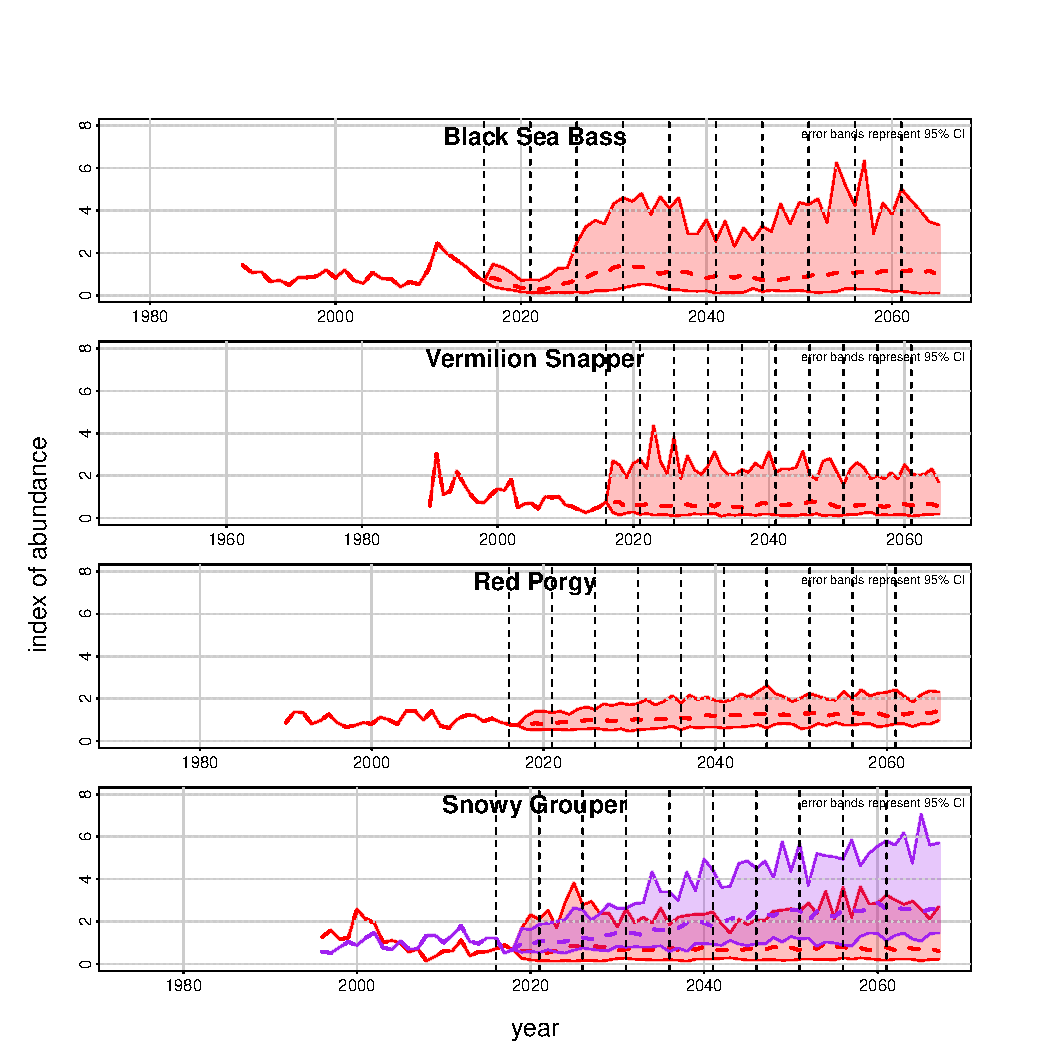
\includegraphics[width=6in,height=7in]{../Figs/AddInd.pdf}
\end{center}
\begin{flushleft}
\caption{Indices derived from BAM stock assessments available during the projection period, for the SCA (10) MP in the Base scenario, where stock assessments are conducted every 10 years during the projection period (dashed vertical lines). Shaded areas represent 95\% CI for indices among simulation runs.}
\label{fig:AddInd}
\end{flushleft}
\end{figure}

\begin{figure}[!ht]
\begin{center}
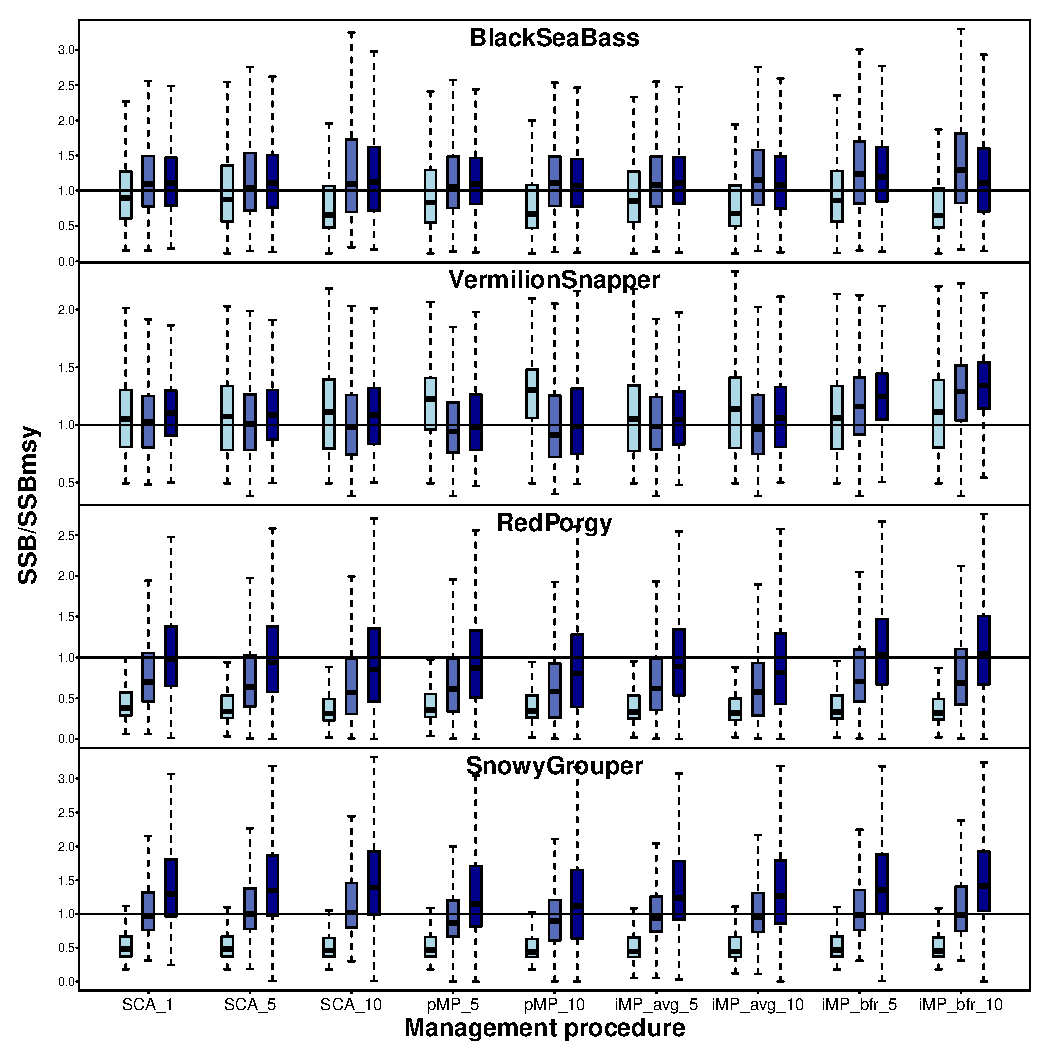
\includegraphics[width=6in, height=7in]{../Figs/boxplotSBSBMSY1.pdf}
\end{center}
\begin{flushleft}
\caption{Box plots of $\mathrm{SSB/SSB_{MSY}}$ for the base scenario. Grouped boxes represent sequential time periods during the projection period. Boxes represent interquartile range (IQR). Whiskers are drawn to $1.5\times\mathrm{IQR}$.}
\label{fig:boxplotSBSBMSY1}
\end{flushleft}
\end{figure}
\clearpage\begin{figure}[!ht]
\begin{center}
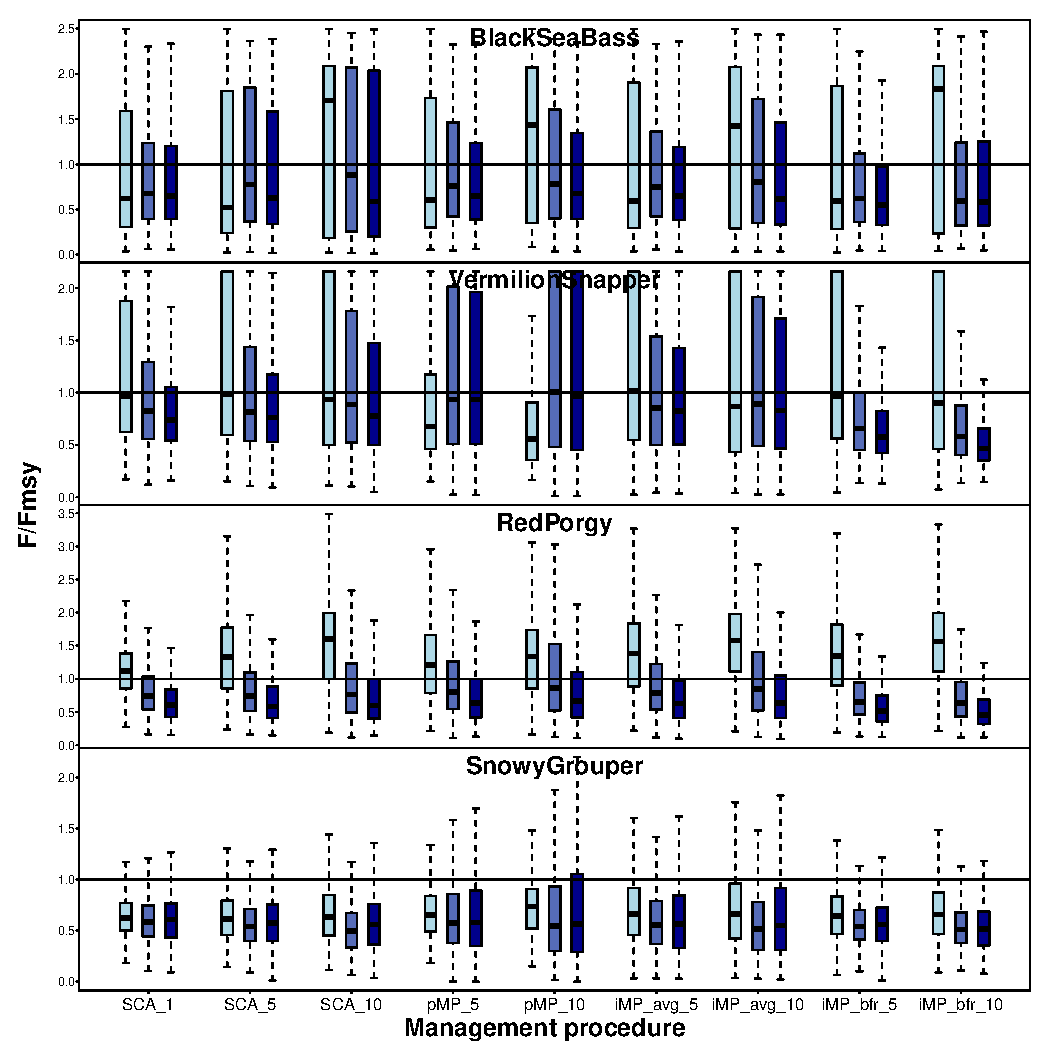
\includegraphics[width=6in, height=7in]{../Figs/boxplotFFMSY1.pdf}
\end{center}
\begin{flushleft}
\caption{Box plots of $\mathrm{F/F_{MSY}}$ for the base scenario. Grouped boxes represent sequential time periods during the projection period. Boxes represent interquartile range (IQR). Whiskers are drawn to $1.5\times\mathrm{IQR}$.}
\label{fig:boxplotFFMSY1}
\end{flushleft}
\end{figure}
\clearpage\begin{figure}[!ht]
\begin{center}
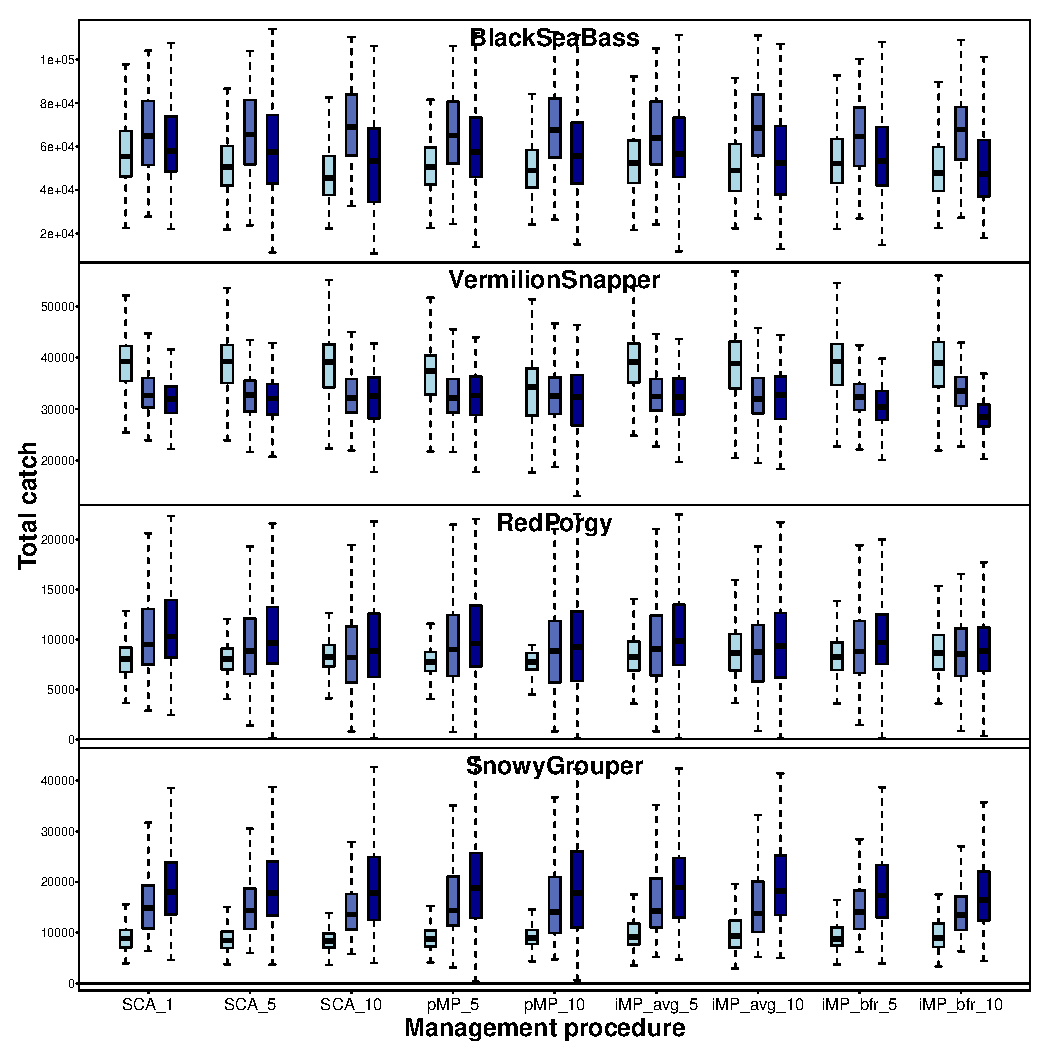
\includegraphics[width=6in, height=7in]{../Figs/boxplotCatchTotal1.pdf}
\end{center}
\begin{flushleft}
\caption{Box plots of total catch (annual catches summed across each time period) for the base scenario. Grouped boxes represent sequential time periods during the projection period. Boxes represent interquartile range (IQR). Whiskers are drawn to $1.5\times\mathrm{IQR}$.}
\label{fig:boxplotCatchTotal1}
\end{flushleft}
\end{figure}
\clearpage\begin{figure}[!ht]
\begin{center}
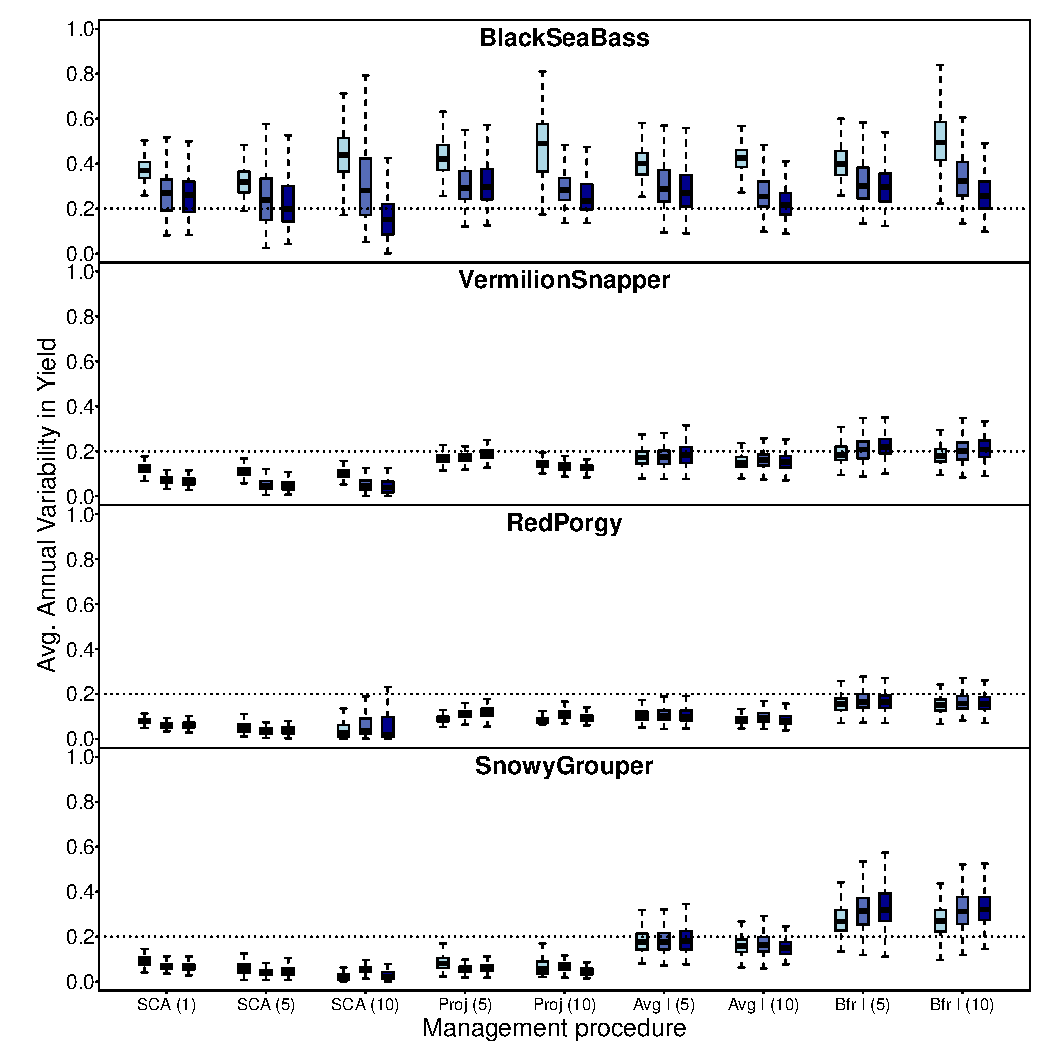
\includegraphics[width=6in, height=7in]{../Figs/boxplotAAVY1.pdf}
\end{center}
\begin{flushleft}
\caption{Box plots of average annual variation in yield ($\mathrm{AAVY}$) for the base scenario. Grouped boxes represent sequential time periods during the projection period. Boxes represent interquartile range (IQR). Whiskers are drawn to $1.5\times\mathrm{IQR}$.}
\label{fig:boxplotAAVY1}
\end{flushleft}
\end{figure}
\clearpage
\begin{figure}[!ht]
\begin{center}
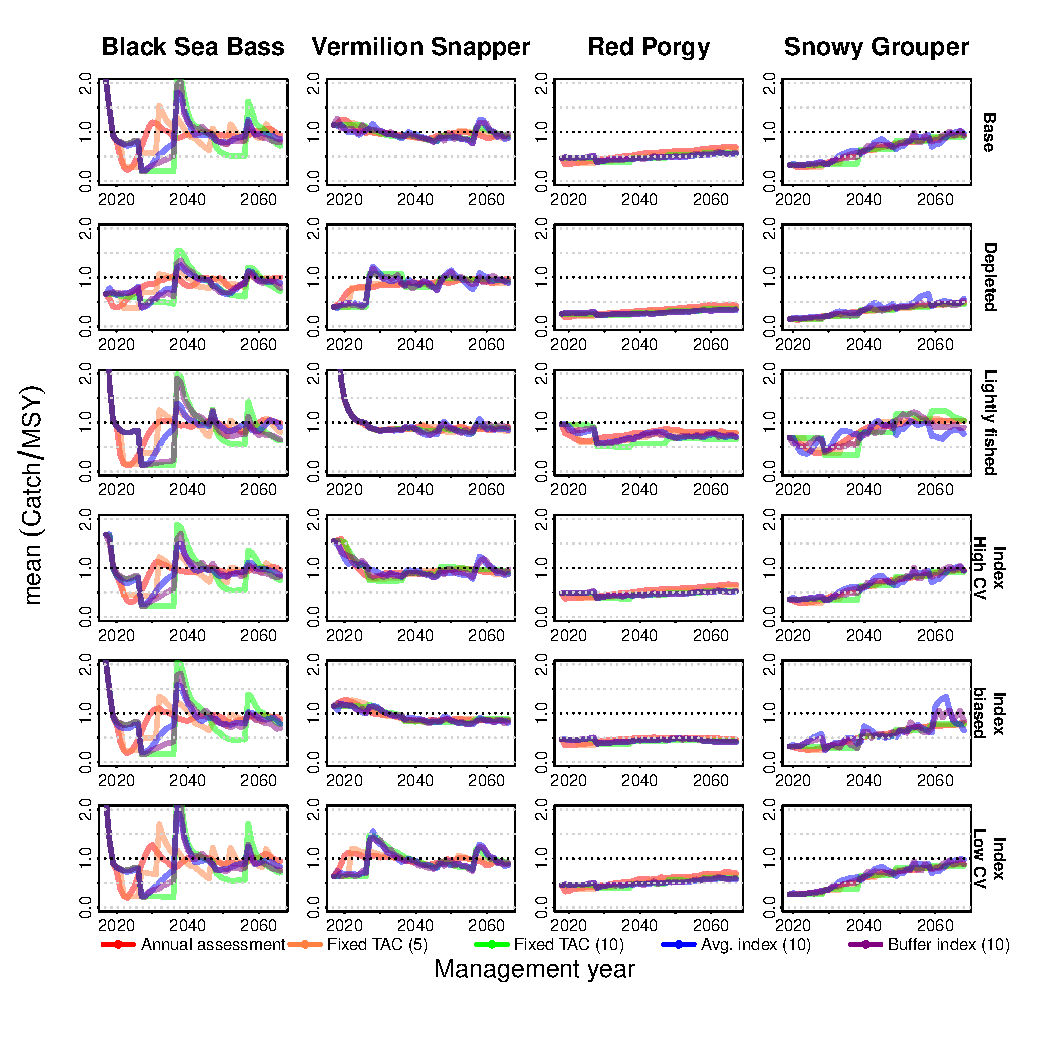
\includegraphics[width=6in, height=7in]{../Figs/tsCatchMSY1.pdf}
\end{center}
\begin{flushleft}
\caption{Time series of median $\mathrm{catch/MSY}$ among simulation runs for the base scenario.Vertical dotted lines indicate assessment years at 10 yr intervals.}
\label{fig:tsCatchMSY1}
\end{flushleft}
\end{figure}
\clearpage\begin{figure}[!ht]
\begin{center}
\includegraphics[width=6in, height=7in]{../Figs/tsCatchMSY1B.pdf}
\end{center}
\begin{flushleft}
\caption{Time series of median $\mathrm{catch/MSY}$ among simulation runs for the base scenario.Vertical dotted lines indicate assessment years at 5 yr intervals.}
\label{fig:tsCatchMSY1B}
\end{flushleft}
\end{figure}
\clearpage\begin{figure}[!ht]
\begin{center}
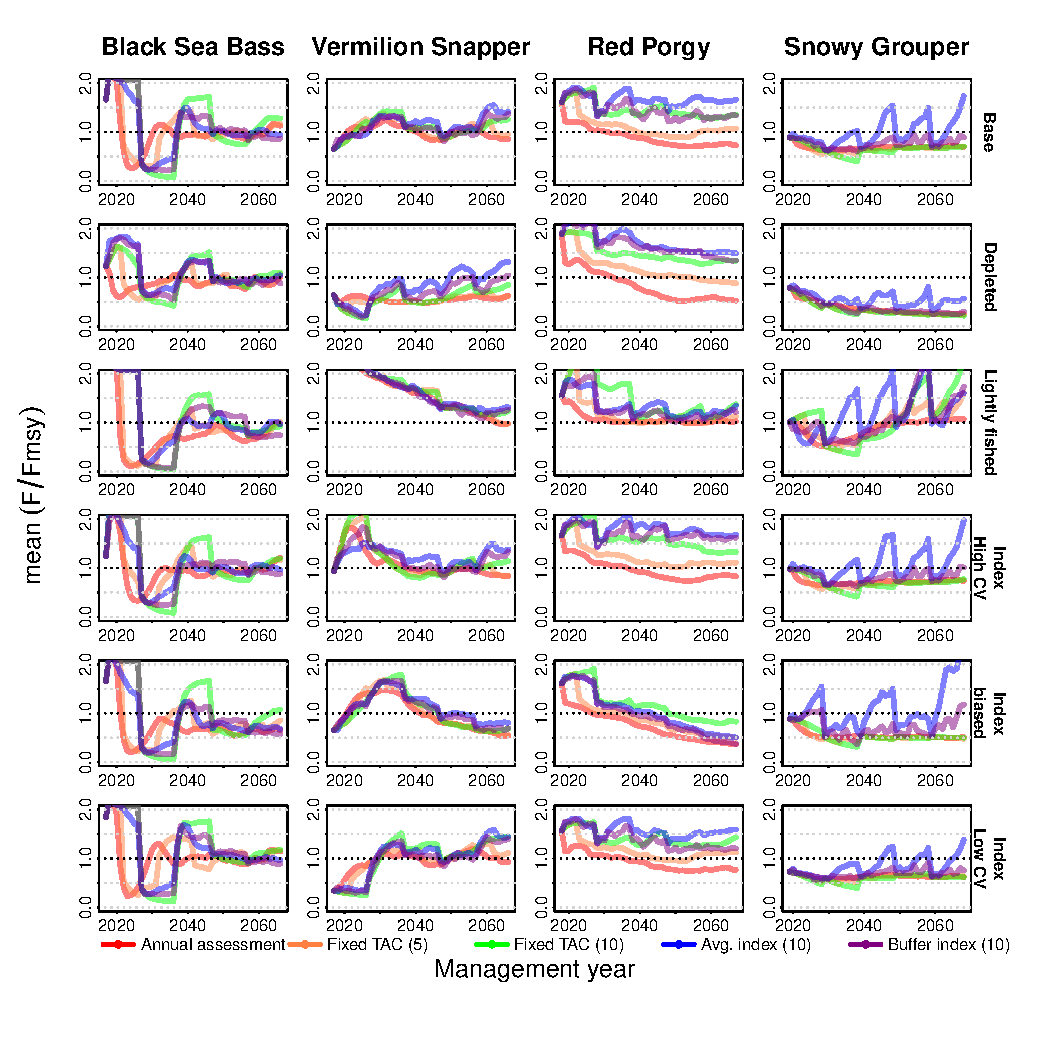
\includegraphics[width=6in, height=7in]{../Figs/tsFFmsy1.pdf}
\end{center}
\begin{flushleft}
\caption{Time series of median $\mathrm{F/F_{MSY}}$ among simulation runs for the base scenario.Vertical dotted lines indicate assessment years at 10 yr intervals.}
\label{fig:tsFFmsy1}
\end{flushleft}
\end{figure}
\clearpage\begin{figure}[!ht]
\begin{center}
\includegraphics[width=6in, height=7in]{../Figs/tsFFmsy1B.pdf}
\end{center}
\begin{flushleft}
\caption{Time series of median $\mathrm{F/F_{MSY}}$ among simulation runs for the base scenario.Vertical dotted lines indicate assessment years at 5 yr intervals.}
\label{fig:tsFFmsy1B}
\end{flushleft}
\end{figure}
\clearpage\begin{figure}[!ht]
\begin{center}
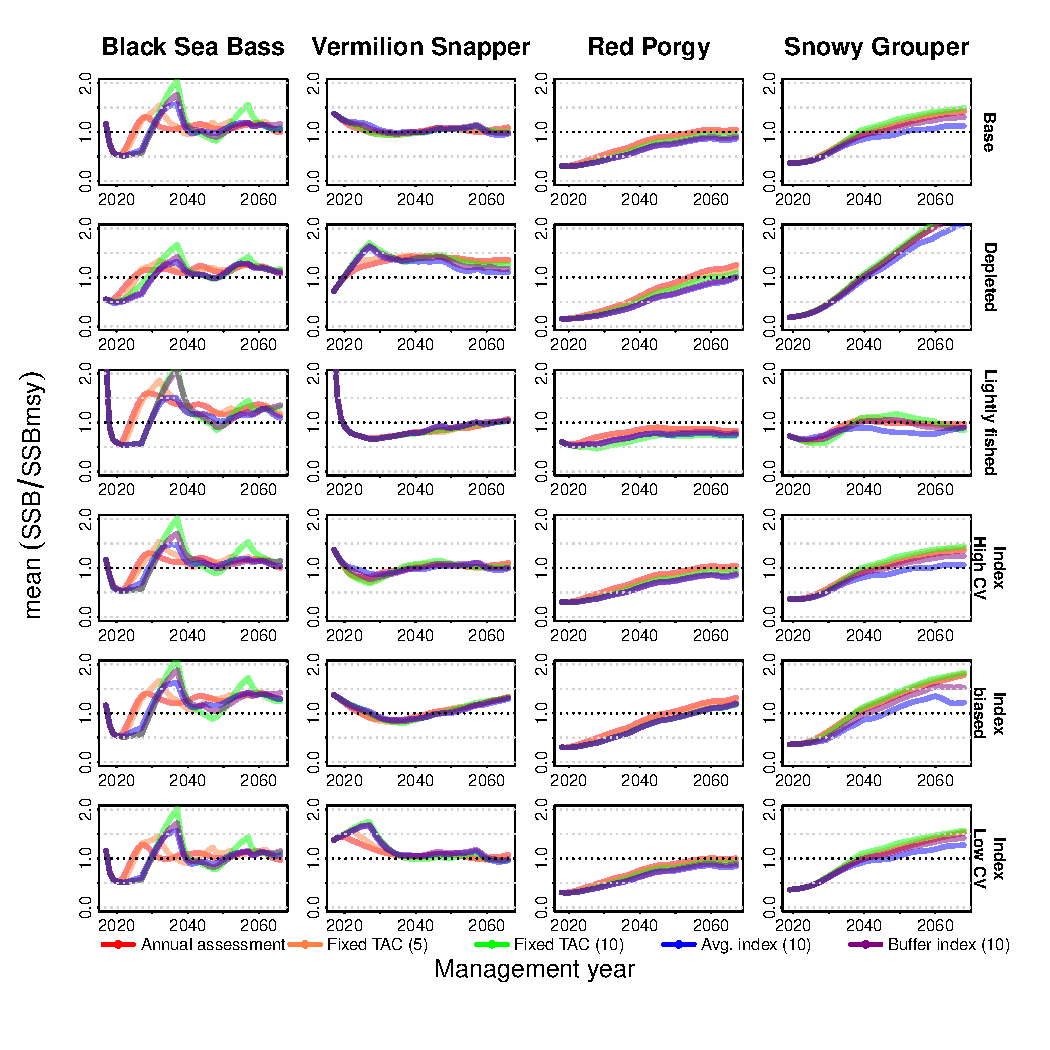
\includegraphics[width=6in, height=7in]{../Figs/tsSSBSSBmsy1.pdf}
\end{center}
\begin{flushleft}
\caption{Time series of median $\mathrm{SSB/SSB_{MSY}}$ among simulation runs for the base scenario.Vertical dotted lines indicate assessment years at 10 yr intervals.}
\label{fig:tsSSBSSBmsy1}
\end{flushleft}
\end{figure}
\clearpage\begin{figure}[!ht]
\begin{center}
\includegraphics[width=6in, height=7in]{../Figs/tsSSBSSBmsy1B.pdf}
\end{center}
\begin{flushleft}
\caption{Time series of median $\mathrm{SSB/SSB_{MSY}}$ among simulation runs for the base scenario.Vertical dotted lines indicate assessment years at 5 yr intervals.}
\label{fig:tsSSBSSBmsy1B}
\end{flushleft}
\end{figure}
\clearpage

\begin{figure}[!ht]
\begin{center}
\includegraphics[width=7in, height=3.5in]{../Figs/trAAVYP1001.pdf}
\end{center}
\begin{flushleft}
\caption{Trade off plots of the probability that average annual variability in yield (AAVY) <20\%, versus  the probability that $\mathrm{SSB > SSB_{MSY}}$ among simulation runs for the base scenario. Plots are based on data for the last 10 years of the projection period.}
\label{fig:trAAVYP1001}
\end{flushleft}
\end{figure}
\clearpage\begin{figure}[!ht]
\begin{center}
\includegraphics[width=7in, height=3.5in]{../Figs/trAAVYPNOF1.pdf}
\end{center}
\begin{flushleft}
\caption{Trade off plots of the probability that average annual variability in yield (AAVY) <20\%, versus  the probability that $\mathrm{F < F_{MSY}}$ among simulation runs for the base scenario. Plots are based on data for the last 10 years of the projection period.}
\label{fig:trAAVYPNOF1}
\end{flushleft}
\end{figure}
\clearpage\begin{figure}[!ht]
\begin{center}
\includegraphics[width=7in, height=3.5in]{../Figs/trAAVYYldLT1.pdf}
\end{center}
\begin{flushleft}
\caption{Trade off plots of the probability that average annual variability in yield (AAVY) <20\%, versus  longterm yield among simulation runs for the base scenario. Plots are based on data for the last 10 years of the projection period.}
\label{fig:trAAVYYldLT1}
\end{flushleft}
\end{figure}
\clearpage\begin{figure}[!ht]
\begin{center}
\includegraphics[width=7in, height=3.5in]{../Figs/trP100YldLT1.pdf}
\end{center}
\begin{flushleft}
\caption{Trade off plots of the probability that $\mathrm{SSB > SSB_{MSY}}$ versus  longterm yield among simulation runs for the base scenario. Plots are based on data for the last 10 years of the projection period.}
\label{fig:trP100YldLT1}
\end{flushleft}
\end{figure}
\clearpage\begin{figure}[!ht]
\begin{center}
\includegraphics[width=7in, height=3.5in]{../Figs/trPNOFP1001.pdf}
\end{center}
\begin{flushleft}
\caption{Trade off plots of the probability that $\mathrm{F < F_{MSY}}$  versus  the probability that $\mathrm{SSB > SSB_{MSY}}$ among simulation runs for the base scenario. Plots are based on data for the last 10 years of the projection period.}
\label{fig:trPNOFP1001}
\end{flushleft}
\end{figure}
\clearpage
\begin{figure}[!ht]
\begin{center}
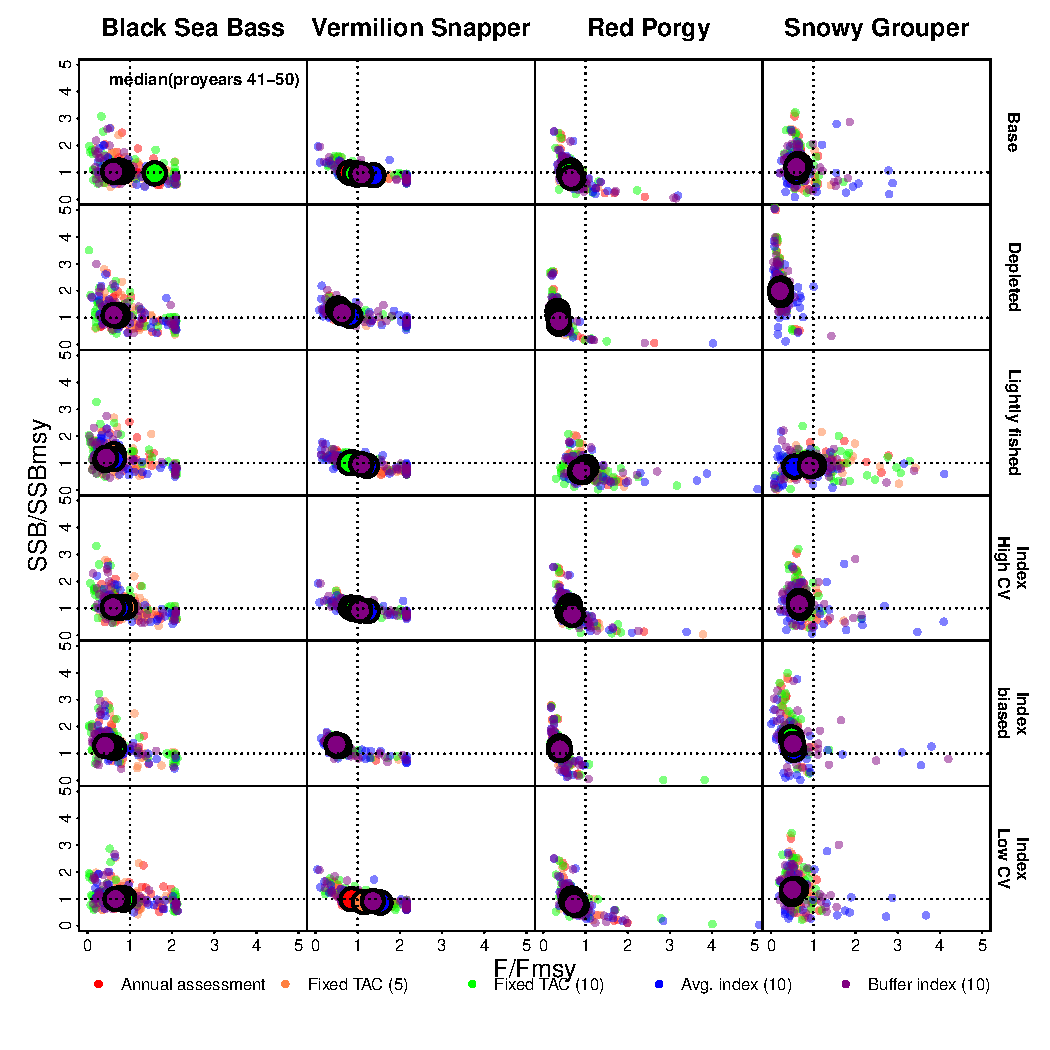
\includegraphics[width=7in, height=3.5in]{../Figs/phasePlot1.pdf}
\end{center}
\begin{flushleft}
\caption{Phase plots of the probability that $\mathrm{F > F_{MSY}}$  versus  the probability that $\mathrm{SSB > SSB_{MSY}}$ among simulation runs for the base scenario.}
\label{fig:phasePlot1}
\end{flushleft}
\end{figure}
\clearpage
%% APPENDIX
\begin{appendix}

\clearpage
\section*{Appendix}

\setcounter{figure}{0}
\renewcommand{\thefigure}{S\arabic{figure}}

% \setcounter{table}{0}
% \renewcommand{\thetable}{S\arabic{table}}
%
% \input{../Results/Appendix.tex}
%
% \input{../Results/biodivByBlock.tex}
%

\begin{figure}[!ht]
\begin{center}
\includegraphics[width=6in, height=7in]{../Figs/boxplotSBSBMSY2.pdf}
\end{center}
\begin{flushleft}
\caption{Box plots of $\mathrm{SSB/SSB_{MSY}}$ for the base and alternative scenarios. Grouped boxes represent sequential time periods during the projection period. Boxes represent interquartile range (IQR). Whiskers are drawn to $1.5\times\mathrm{IQR}$.}
\label{fig:boxplotSBSBMSY2}
\end{flushleft}
\end{figure}
\clearpage\begin{figure}[!ht]
\begin{center}
\includegraphics[width=6in, height=7in]{../Figs/boxplotFFMSY2.pdf}
\end{center}
\begin{flushleft}
\caption{Box plots of $\mathrm{F/F_{MSY}}$ for the base and alternative scenarios. Grouped boxes represent sequential time periods during the projection period. Boxes represent interquartile range (IQR). Whiskers are drawn to $1.5\times\mathrm{IQR}$.}
\label{fig:boxplotFFMSY2}
\end{flushleft}
\end{figure}
\clearpage\begin{figure}[!ht]
\begin{center}
\includegraphics[width=6in, height=7in]{../Figs/boxplotCatchTotal2.pdf}
\end{center}
\begin{flushleft}
\caption{Box plots of total catch (annual catches summed across each time period) for the base and alternative scenarios. Grouped boxes represent sequential time periods during the projection period. Boxes represent interquartile range (IQR). Whiskers are drawn to $1.5\times\mathrm{IQR}$.}
\label{fig:boxplotCatchTotal2}
\end{flushleft}
\end{figure}
\clearpage\begin{figure}[!ht]
\begin{center}
\includegraphics[width=6in, height=7in]{../Figs/boxplotAAVY2.pdf}
\end{center}
\begin{flushleft}
\caption{Box plots of average annual variation in yield ($\mathrm{AAVY}$) for the base and alternative scenarios. Grouped boxes represent sequential time periods during the projection period. Boxes represent interquartile range (IQR). Whiskers are drawn to $1.5\times\mathrm{IQR}$.}
\label{fig:boxplotAAVY2}
\end{flushleft}
\end{figure}
\clearpage
\begin{figure}[!ht]
\begin{center}
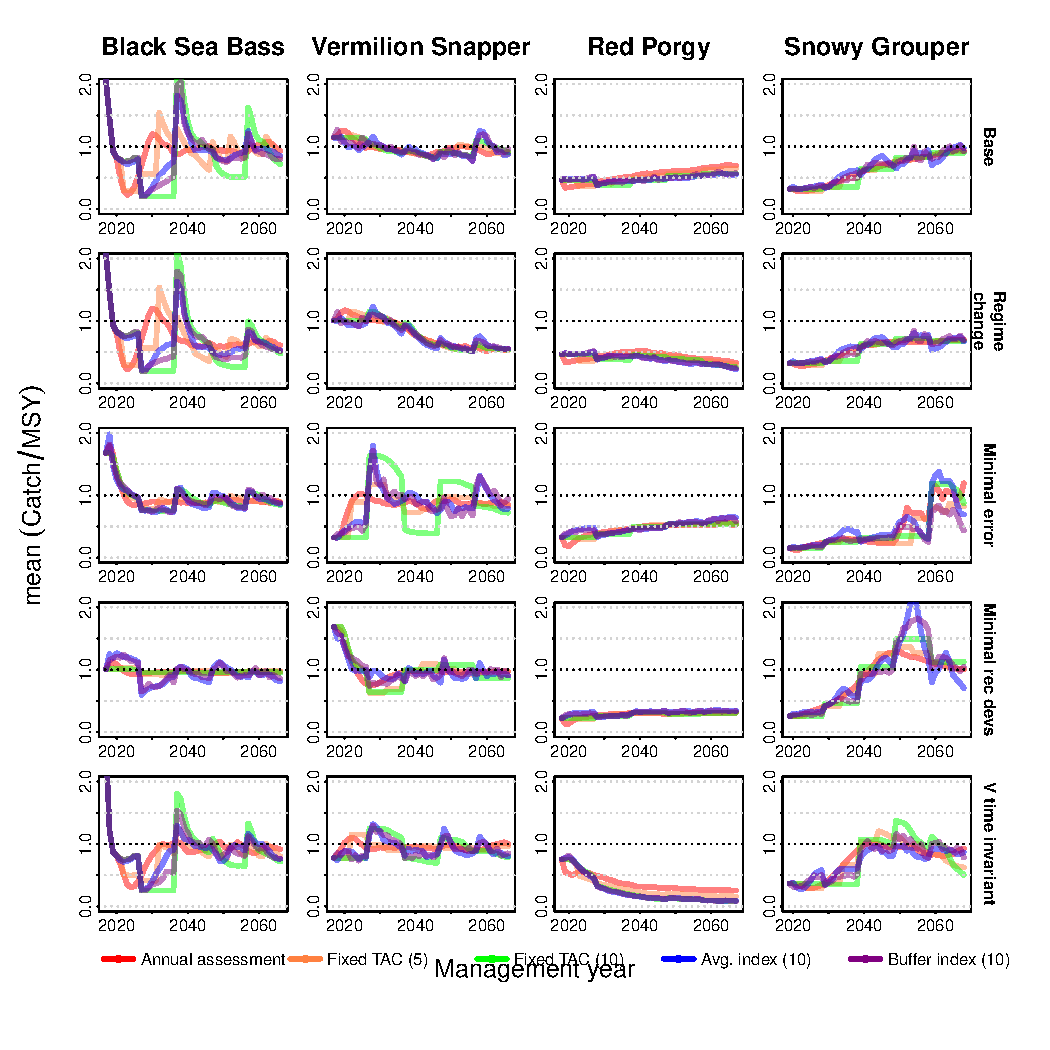
\includegraphics[width=6in, height=7in]{../Figs/tsCatchMSY2.pdf}
\end{center}
\begin{flushleft}
\caption{Time series of median $\mathrm{catch/MSY}$ among simulation runs for the base scenario.Vertical dotted lines indicate assessment years at 10 yr intervals.}
\label{fig:tsCatchMSY2}
\end{flushleft}
\end{figure}
\clearpage\begin{figure}[!ht]
\begin{center}
\includegraphics[width=6in, height=7in]{../Figs/tsCatchMSY2B.pdf}
\end{center}
\begin{flushleft}
\caption{Time series of median $\mathrm{catch/MSY}$ among simulation runs for the base scenario.Vertical dotted lines indicate assessment years at 5 yr intervals.}
\label{fig:tsCatchMSY2B}
\end{flushleft}
\end{figure}
\clearpage\begin{figure}[!ht]
\begin{center}
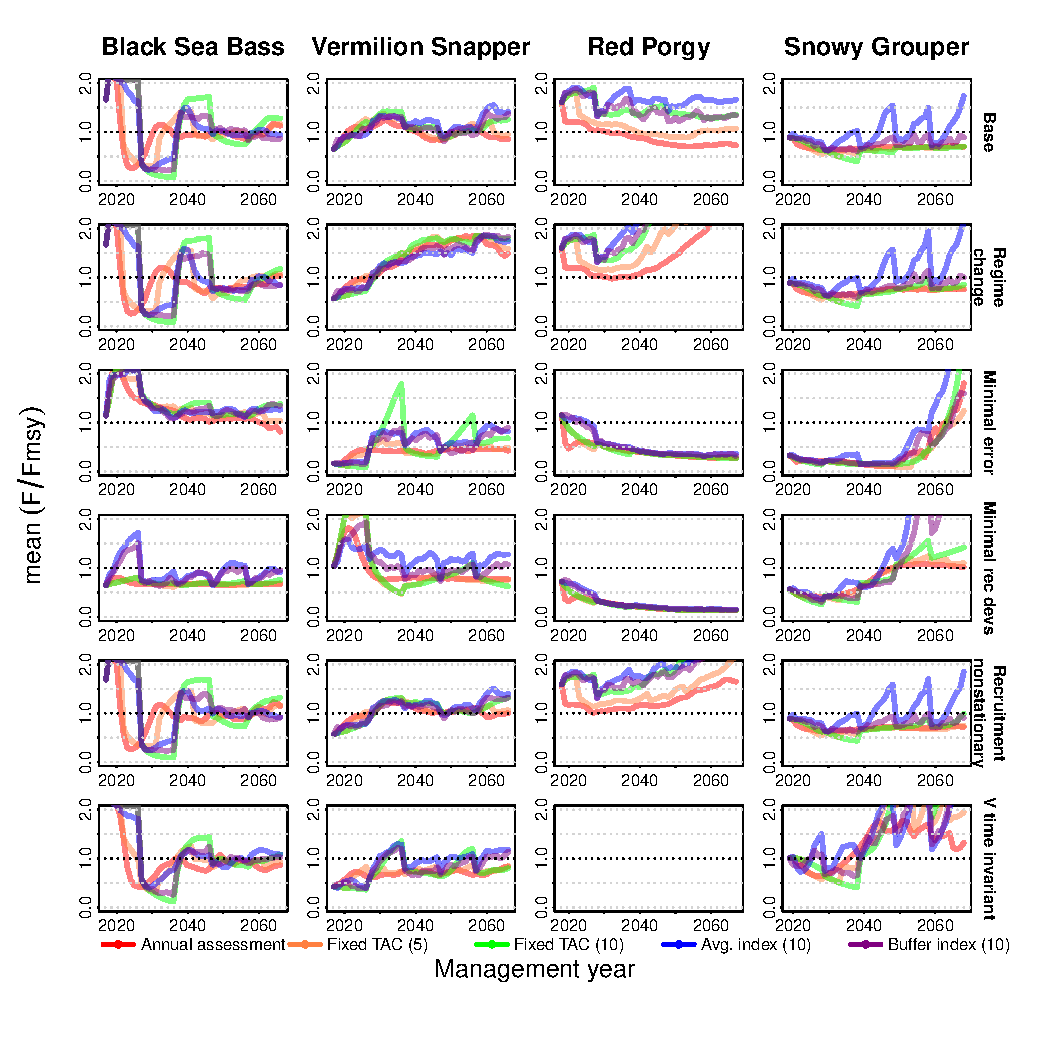
\includegraphics[width=6in, height=7in]{../Figs/tsFFmsy2.pdf}
\end{center}
\begin{flushleft}
\caption{Time series of median $\mathrm{F/F_{MSY}}$ among simulation runs for the base scenario.Vertical dotted lines indicate assessment years at 10 yr intervals.}
\label{fig:tsFFmsy2}
\end{flushleft}
\end{figure}
\clearpage\begin{figure}[!ht]
\begin{center}
\includegraphics[width=6in, height=7in]{../Figs/tsFFmsy2B.pdf}
\end{center}
\begin{flushleft}
\caption{Time series of median $\mathrm{F/F_{MSY}}$ among simulation runs for the base scenario.Vertical dotted lines indicate assessment years at 5 yr intervals.}
\label{fig:tsFFmsy2B}
\end{flushleft}
\end{figure}
\clearpage\begin{figure}[!ht]
\begin{center}
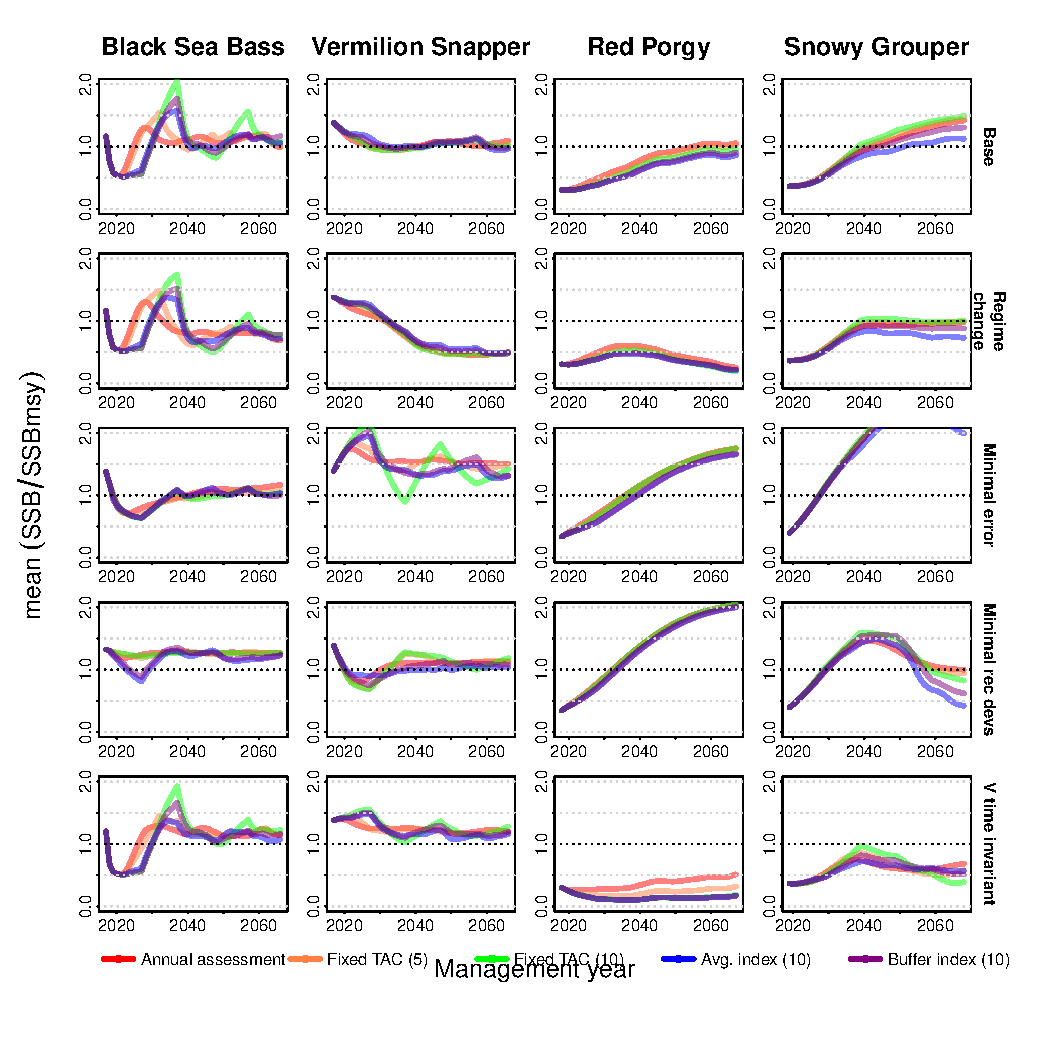
\includegraphics[width=6in, height=7in]{../Figs/tsSSBSSBmsy2.pdf}
\end{center}
\begin{flushleft}
\caption{Time series of median $\mathrm{SSB/SSB_{MSY}}$ among simulation runs for the base scenario.Vertical dotted lines indicate assessment years at 10 yr intervals.}
\label{fig:tsSSBSSBmsy2}
\end{flushleft}
\end{figure}
\clearpage\begin{figure}[!ht]
\begin{center}
\includegraphics[width=6in, height=7in]{../Figs/tsSSBSSBmsy2B.pdf}
\end{center}
\begin{flushleft}
\caption{Time series of median $\mathrm{SSB/SSB_{MSY}}$ among simulation runs for the base scenario.Vertical dotted lines indicate assessment years at 5 yr intervals.}
\label{fig:tsSSBSSBmsy2B}
\end{flushleft}
\end{figure}
\clearpage
\begin{figure}[!ht]
\begin{center}
\includegraphics[width=7in, height=8in]{../Figs/trAAVYP1002.pdf}
\end{center}
\begin{flushleft}
\caption{Trade off plots of the probability that average annual variability in yield (AAVY) <20\%, versus  the probability that $\mathrm{SSB > SSB_{MSY}}$ among simulation runs for the base and alternative scenarios. Plots are based on data for the last 10 years of the projection period.}
\label{fig:trAAVYP1002}
\end{flushleft}
\end{figure}
\clearpage\begin{figure}[!ht]
\begin{center}
\includegraphics[width=7in, height=8in]{../Figs/trAAVYPNOF2.pdf}
\end{center}
\begin{flushleft}
\caption{Trade off plots of the probability that average annual variability in yield (AAVY) <20\%, versus  the probability that $\mathrm{F > F_{MSY}}$ among simulation runs for the base and alternative scenarios. Plots are based on data for the last 10 years of the projection period.}
\label{fig:trAAVYPNOF2}
\end{flushleft}
\end{figure}
\clearpage\begin{figure}[!ht]
\begin{center}
\includegraphics[width=7in, height=8in]{../Figs/trAAVYYldLT2.pdf}
\end{center}
\begin{flushleft}
\caption{Trade off plots of the probability that average annual variability in yield (AAVY) <20\%, versus  longterm yield among simulation runs for the base and alternative scenarios. Plots are based on data for the last 10 years of the projection period.}
\label{fig:trAAVYYldLT2}
\end{flushleft}
\end{figure}
\clearpage\begin{figure}[!ht]
\begin{center}
\includegraphics[width=7in, height=8in]{../Figs/trPNOFP1002.pdf}
\end{center}
\begin{flushleft}
\caption{Trade off plots of the probability that $\mathrm{F > F_{MSY}}$  versus  the probability that $\mathrm{SSB > SSB_{MSY}}$ among simulation runs for the base and alternative scenarios. Plots are based on data for the last 10 years of the projection period.}
\label{fig:trPNOFP1002}
\end{flushleft}
\end{figure}
\clearpage
\begin{figure}[!ht]
\begin{center}
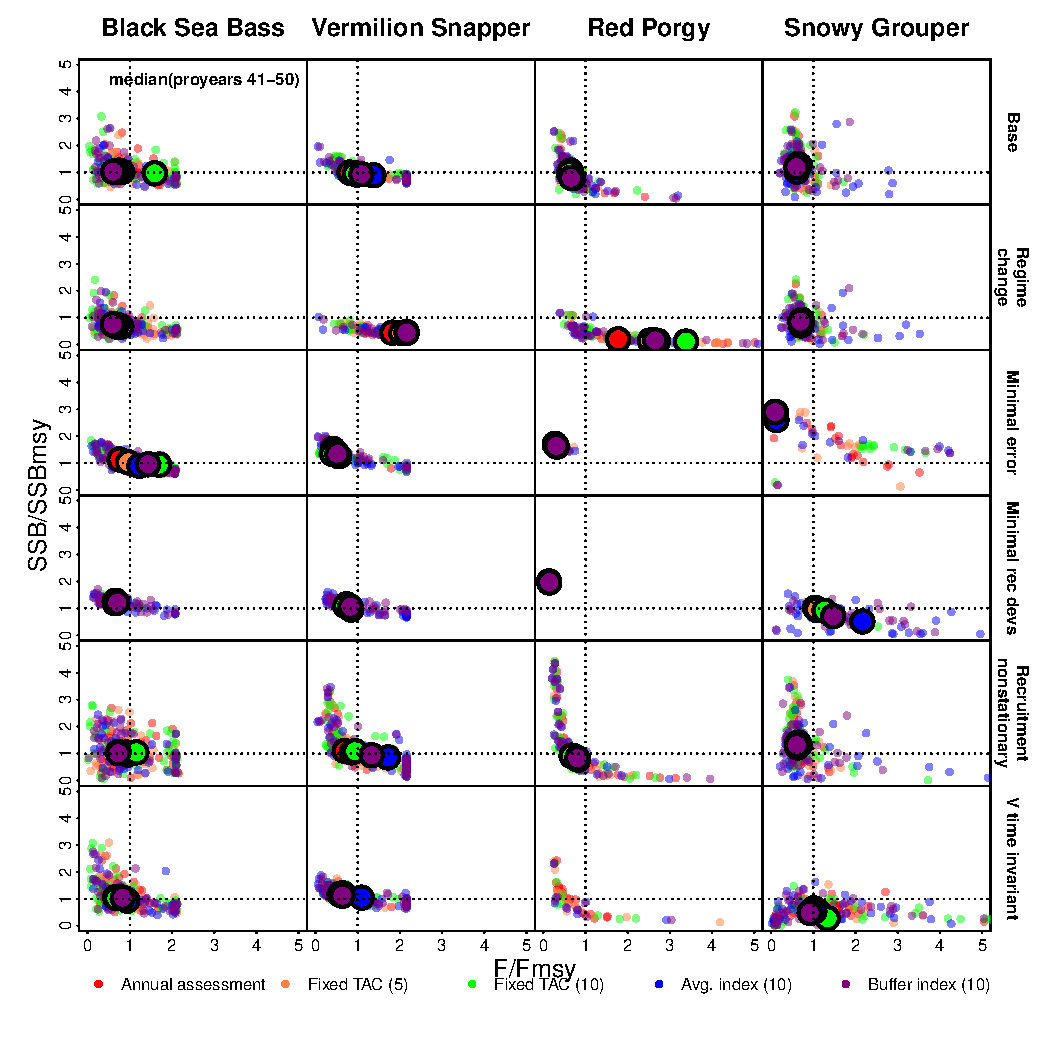
\includegraphics[width=7in, height=8in]{../Figs/phasePlot2.pdf}
\end{center}
\begin{flushleft}
\caption{Phase plots of the probability that $\mathrm{F > F_{MSY}}$  versus  the probability that $\mathrm{SSB > SSB_{MSY}}$ among simulation runs for the base and alternative scenarios.}
\label{fig:phasePlot2}
\end{flushleft}
\end{figure}
\clearpage

\end{appendix}


% END DOCUMENT
\end{document}
